\documentclass[titlepage, a4paper]{article}
\usepackage[swedish]{babel}
\usepackage[utf8]{inputenc}
\usepackage{graphicx}
\usepackage{color}
\usepackage{mathtools}
\usepackage{etoolbox}
\usepackage{caption}
\usepackage{float}
\usepackage{listings}
% Sidformat
\usepackage{a4wide}
\usepackage[parfill]{parskip}
% Bättre bildtexter
\usepackage[margin=10pt,font=small,labelfont=bf,labelsep=endash]{caption}

% Enkelt kommando som låter mig attgöra-markera text
\newcommand{\todo}[1] {\textbf{\textcolor{red}{#1}}}

\usepackage{graphicx,epstopdf}
\usepackage{listings}
\epstopdfsetup{suffix=}
\DeclareGraphicsExtensions{.ps}
\DeclareGraphicsRule{.ps}{pdf}{.pdf}{`ps2pdf -dEPSCrop -dNOSAFER #1 \noexpand\OutputFile}

\lstset{literate=%
    {å}{{\r{a}}}1
    {ä}{{\"a}}1
    {ö}{{\"o}}1
    {Å}{{\r{A}}}1
    {Ä}{{\"A}}1
    {Ö}{{\"O}}1
}

%% Headers och Footers
\usepackage{fancyhdr}
\pagestyle{fancy}
\rhead{Martin Söderén \\ Alexander Yngve}
\chead{TANA21}

\begin{document}

{\ }\vspace{45mm}

\begin{center}
    \Huge \textbf{TANA21: Projektrapport}
\end{center}
\begin{center}
    \Large Numerisk linjär algebra
\end{center}

\vspace{250pt}

\begin{center}
    \begin{tabular}{|*{3}{p{40mm}|}}
        \hline
        \textbf{Namn} & \textbf{Personnummer} & \textbf{Epostaddress} \\ \hline
        {Martin Söderén} & {900929-1098} & {marso329@student.liu.se} \\ \hline
        {Alexander Yngve} & {930320-6651} & {aleyn573@student.liu.se} \\ \hline
    \end{tabular}
\end{center}
\newpage

\section{Inledning}
Denna rapport behandlar hur man kan lösa polynom approximationer med hjälp av MATLAB och Newtons metod för approximation och vilka resultat man kan förvänta sig.

\section{Uppgift}
Projektets uppgift är att skapa två MATLAB-funktioner, mypolyfit som bestämmer ett interpolationspolynom av lägsta möjliga grad och mypolyval som som evaluerar det beräknade polynomet. Därefter ska den förstnämnda funktionens korrekthet kontrolleras och dess tidskomplexitet bestämmas.
\newline
\newline
Frågor att besvara:
\begin{itemize}
\item Räknar koderna rätt?
\item Är kodernas aritmetiska komplexitet som förväntad?
\end{itemize}


\section{Teori}\label{sec:teori}
Enligt sats 5.2.1 i kursboken så går det att bestämma ett entydigt polynom av grad $\leq$ n om det finns n+1 skilda punkter.
\newline
\newline
Genom att ansätta ett interpolationspolynom kan man skapa ett linjärt ekvationssystem.  Detta kan man sätta upp i matrisform och då blir koefficientmatrisen triangulerad vilket leder till att denna kan lösas med antingen framåtsubstitution eller bakåtsubstitution. Detta ger tidskomplexiteten $\mathcal{O}(n^2)$ enligt kursbok kapitel 5.4. 


\begin{figure}[H]
  $$f[x_i]=f(x_i)$$
  $$f[x_1,x_1......,x_{k+1}]=\dfrac{f[x_2,x_3,....,x_{k+1}]-f[x_1,x_2,....,x_{k}]}{x_{k+1} -x_1}$$ 
  \caption*{Den k:te dividerade differensen av f}
\end{figure}
För utvärdering av polynom så används Horners schema som beskrivs i kursboken avsnitt 4.6. Fördeled med Horners är att den beräknar polynomet rekursivt och använder hälften som många multiplikationer jämfört med med om man evaluerar polynomet normalt.

\section{Metod}\label{sec:metod}
Funktionerna implementerades enligt metoden beskriven i avsnitt 5.4 i kursboken. Därefter testades \textit{mypolyfit} med koden i figur \ref{lst:test}.

\begin{figure}[H]
  \begin{lstlisting}
%clf;
for i = [5 10 20 40 80 160 320 640 1280]
    N = i;
    x = 1:N;
    y = randi([-20,20], 1, N);

    i
    tic;
    P = mypolyfit(x, y);
    toc;

    px = 1:0.1:N;
    py = mypolyval(P, 1:0.1:N);

    %plot(x, y, '*', px, py);
    %pause;
end
  \end{lstlisting}
  \caption{Testkod}
  \label{lst:test}
\end{figure}



\section{Kod}
Funktionen \textit{mypolyfit} (figur \ref{lst:fit})  bestämmer ett interpolationspolynom av lägsta möjliga grad  och \textit{mypolyval} (figur \ref{lst:val}) evaluerar interpolationspolynomet.

\begin{figure}[H]
  \begin{lstlisting}
function [n] = mypolyfit(x,y)
N = length(x)-1;
temp = zeros(N + 1,N + 1);
temp(1:N + 1,1) = y';
% Create difference table
for k=2:N+1
    for m=1:N+2-k
        temp(m,k) = (temp(m + 1,k - 1) - temp(m,k - 1))/(x(m + k - 1)- x(m));
    end
end
% First row in difference table (def 5.4.1)
a = temp(1,:);
n = a(N+1);
% Nested multiplication for coefficients
for k = N:-1:1 
n = [n a(k)] - [0 n*x(k)];
end
  \end{lstlisting}
  \caption{\textit{mypolyfit}}
  \label{lst:fit}
\end{figure}

\begin{figure}[H]
  \begin{lstlisting}
function [ p ] = mypolyval( P, X )
n=length(P)-1;
p=P(1);
for i=1:n
    p=p.*X+P(i+1);
end
  \end{lstlisting}
  \caption{\textit{mypolyval}}
  \label{lst:val}
\end{figure}


\section{Validering}
Om man väljer att plotta figurer i koden i figur \ref{lst:test} så ser man att alla punkter från polynomet ligger på den ursprungliga linjen. Vilket leder till att man kan anta att koden räknar rätt.

\section{Resultat}
Resultatet av testet beskrivet i avsnitt \ref{sec:metod} återges i tabell \ref{tab:resultat}.

\begin{table}[H]
  \centering
  \begin{tabular}{|l|l|}
    \hline
    \textbf{Datapunkter} & \textbf{Tid (s)} \\ \hline
    5 &0.000160 \\ \hline
    10 & 0.000244 \\ \hline
    20 & 0.000448 \\ \hline
    40 & 0.000787 \\ \hline
    80 & 0.000683 \\ \hline
    160 & 0.001644 \\ \hline
    320 & 0.005802 \\ \hline
    640 & 0.015361 \\ \hline
    1280 & 0.060299 \\ \hline
  \end{tabular}
  \caption{Resultat}
  \label{tab:resultat}
\end{table}
\begin{figure}[h]
  \centering
  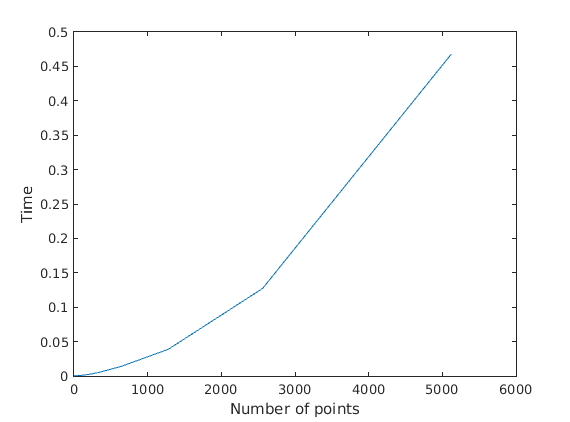
\includegraphics[scale=0.5]{plot.png}
  \caption{Tiden plottad.}
  \label{fig:sten}
\end{figure}
\section{Diskussion}
Vi har kört testkoden många gånger och inte fått ett fel någon gång så vi antar att koden räknar rätt. Vad gäller tidskomplexiteten så är datan väldigt ostabil vilket leder till att det är svårt att avgöra vilken tidskomplexitet den har men den verkar vara $\mathcal{O}(n^2)$ vilket är som förväntat.
\end{document}

